\documentclass{article}

\usepackage{tikz}
\usetikzlibrary{mindmap,trees,backgrounds}
\begin{document}
\pagestyle{empty}
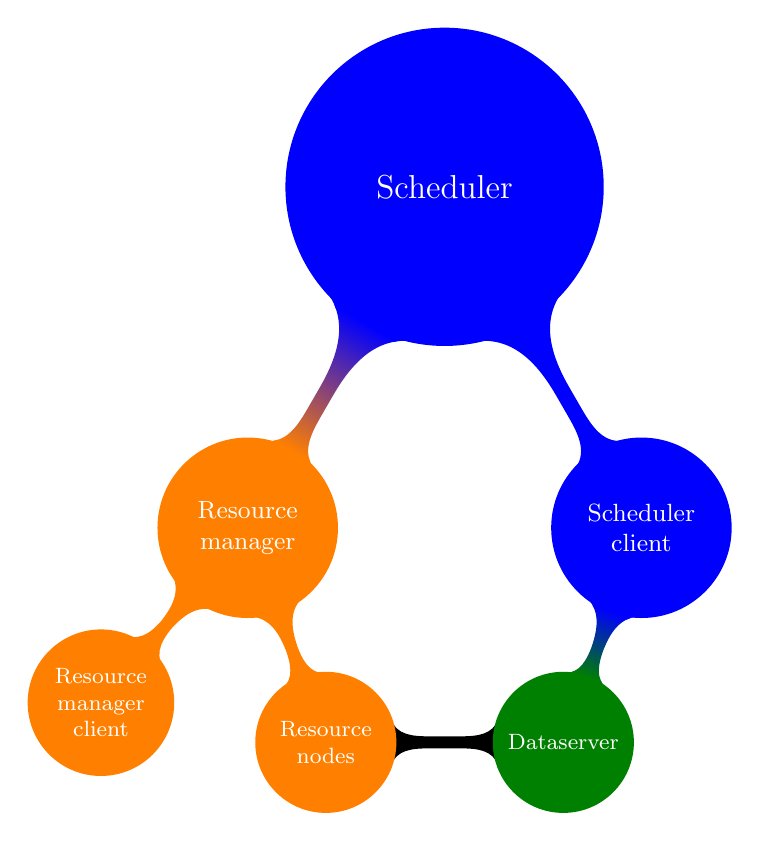
\begin{tikzpicture}
  \path[mindmap,concept color=blue,text=white]
    node[concept] {Scheduler}
    [clockwise from=-60]
    child {
      node[concept] {Scheduler client}
      [clockwise from=-110]
      child [concept color=green!50!black] { node[concept] (pad) {Dataserver} }
    }  
    child[concept color=orange] {
      node[concept] {Resource manager}
      [clockwise from=-70]
      child { node[concept] (node) {Resource nodes} }
      child { node[concept] {Resource manager client} }
    };

    \begin{pgfonlayer}{background}
        %\draw [draw=green!50!black,fill=orange, decorate,decoration=circle connection bar]
        %(pad) -- (node);
        \path (node) to[color=orange, circle connection bar] (pad);
    \end{pgfonlayer}

\end{tikzpicture}\end{document}
